\section{Full Environment Results}


In the full environment description, we generally evaluated the performance of variants of the SAC algorithm. We tested with different perception pipeline, different reward definition, and buffer size. Contrary to the simplified environment, we verified the algorithm's robustness on the wooden block object database.

We tested four variations of the SAC model in the full environment: encoder with fifty thousand buffer size, encoder with one million buffer size, depth with one million buffer size, and RGBD with one million buffer size. Among these models, the encoder one million buffer achieved the best transfer result. It performed with 99\% and 82\% with random objects and wooden blocks in the table scene \ref{table:SACfull}. Nevertheless, training plots demonstrate that the encoder training process has more variance than the depth counterpart. Moreover, depth perception converged to a higher success rate than encoder perception during training, as shown in the plot \ref{fig:percep}.

Like the simplified environment results, we also found that in the full environment, one million buffer size performs better and accumulates less variance than the fifty thousand buffer. As represented in the plot \ref{fig:encbuffer}, the fifty thousand buffer version had more variance and converged to only a 90\% training success rate. In comparison, the one million buffer size version accumulated less variance and converged around a 97\% success rate.  

Unexpectedly, depth perception also performed better than the RGBD. RGBD perception delivered the worst results among perception types. It converged to a 91\% test success rate even in the floor scene. In the same scene, depth perception achieved a 100\% test success rate. RGBD plot in figure \ref{fig:depthvsrgbd} also shows sudden changes, a sign of high variance. Nevertheless, it still converged to a 99\% success rate.

Unfortunately, BDQ never delivered a working policy for the full environment. Its learning plot \ref{fig:bdq} also shows the severe decay to a 0\% success rate.

\begin{table}[!htbp]
    \begin{tabular}{l|l|l|l|l|}
    \cline{2-5}
                                  & \multicolumn{4}{c|}{\textbf{SAC Full Environment}}                                                                                                                                                                                                                                                                                                                                  \\ \cline{2-5}
                                  & \multicolumn{2}{c|}{\textbf{Floor Scene}}                                                                                                                                                & \multicolumn{2}{c|}{\textbf{Table Scene}}                                                                                                                                                \\ \hline
    \multicolumn{1}{|l|}{\textbf{Models}}               & \multicolumn{1}{c|}{\textbf{\begin{tabular}[c]{@{}c@{}}Random Obj. \\ (\%)\end{tabular}}} & \multicolumn{1}{c|}{\textbf{\begin{tabular}[c]{@{}c@{}}Wooden Obj.\\ (\%)\end{tabular}}} & \multicolumn{1}{c|}{\textbf{\begin{tabular}[c]{@{}c@{}}Random Obj. \\ (\%)\end{tabular}}} & \multicolumn{1}{c|}{\textbf{\begin{tabular}[c]{@{}c@{}}Wooden Obj.\\ (\%)\end{tabular}}} \\ \hline
    \multicolumn{1}{|l|}{\textbf{SAC\_encoder\_50k}}    & 65                                                                                          & 62                                                                                         & 63                                                                                          & 59                                                                                         \\ \hline
    \multicolumn{1}{|l|}{\textbf{SAC\_encoder\_1m}}     & 100                                                                                         & 95                                                                                         & 99                                                                                          & 82                                                                                         \\ \hline
    \multicolumn{1}{|l|}{\textbf{SAC\_depth}}           & 100                                                                                         & 95                                                                                         & 95                                                                                          & 23                                                                                         \\ \hline
    \multicolumn{1}{|l|}{\textbf{SAC\_rgbd}}            & 91                                                                                          & 95                                                                                         & 46                                                                                          & 17                                                                                         \\ \hline
    \multicolumn{1}{|l|}{\textbf{SAC\_depth\_sparse}}  & 99                                                                                          & 97                                                                                         & 100                                                                                         & 72                                                                                         \\ \hline
    \multicolumn{1}{|l|}{\textbf{SAC\_depth\_no\_curr}} & 100                                                                                         & 97                                                                                         & 97                                                                                          & 64                                                                                         \\ \hline
    \multicolumn{1}{|l|}{\textbf{SAC\_depth\_no\_act}}  & 95                                                                                          & 75                                                                                         & 84                                                                                          & 24                                                                                         \\ \hline
\end{tabular}
\caption{SAC Full environment results \label{table:SACfull}}
\end{table}


\begin{table}[]
    \begin{tabular}{l|l|l|l|l|l|}
    \cline{2-6}
                                                        & \multicolumn{5}{c|}{\textbf{SAC Full Environment}}                                                                                                                                                                                                                                                                                                                                                                                                                                             \\ \cline{2-6} 
                                                        & \multicolumn{2}{c|}{\textbf{Floor Scene}}                                                                                                                                                & \multicolumn{3}{c|}{\textbf{Table Scene}}                                                                                                                                                                                                                                                           \\ \hline
    \multicolumn{1}{|l|}{\textbf{Models}}               & \multicolumn{1}{c|}{\textbf{\begin{tabular}[c]{@{}c@{}}Random Objects\\ (\%)\end{tabular}}} & \multicolumn{1}{c|}{\textbf{\begin{tabular}[c]{@{}c@{}}Wooden Blocks\\ (\%)\end{tabular}}} & \multicolumn{1}{c|}{\textbf{\begin{tabular}[c]{@{}c@{}}Random Objects\\ (\%)\end{tabular}}} & \multicolumn{1}{c|}{\textbf{\begin{tabular}[c]{@{}c@{}}KUKA Robot\\ Random Objects\\ (\%)\end{tabular}}} & \multicolumn{1}{c|}{\textbf{\begin{tabular}[c]{@{}c@{}}Wooden Blocks\\ (\%)\end{tabular}}} \\ \hline
    \multicolumn{1}{|l|}{\textbf{SAC\_encoder\_50k}}    & 65                                                                                          & 62                                                                                         & 63                                                                                          & 31                                                                                                       & 59                                                                                         \\ \hline
    \multicolumn{1}{|l|}{\textbf{SAC\_encoder\_1m}}     & 100                                                                                         & 95                                                                                         & 99                                                                                          & 87\%                                                                                                     & 82                                                                                         \\ \hline
    \multicolumn{1}{|l|}{\textbf{SAC\_depth}}           & 100                                                                                         & 95                                                                                         & 95                                                                                          & 97\%                                                                                                     & 23                                                                                         \\ \hline
    \multicolumn{1}{|l|}{\textbf{SAC\_rgbd}}            & 91                                                                                          & 95                                                                                         & 46                                                                                          & 38\%                                                                                                     & 17                                                                                         \\ \hline
    \multicolumn{1}{|l|}{\textbf{SAC\_depth\_no\_curr}} & 100                                                                                         & 97                                                                                         & 97                                                                                          & 90\%                                                                                                     & 64                                                                                         \\ \hline
    \multicolumn{1}{|l|}{\textbf{SAC\_depth\_sparse}}   & 99                                                                                          & 97                                                                                         & 100                                                                                         & 28\%                                                                                                     & 72                                                                                         \\ \hline
    \multicolumn{1}{|l|}{\textbf{SAC\_depth\_no\_act}}  & 95                                                                                          & 75                                                                                         & 84                                                                                          & 12                                                                                                       & 24                                                                                         \\ \hline
    \end{tabular}
\end{table}

\begin{figure}[!htbp]
    \begin{subfigure}{0.49\textwidth}
        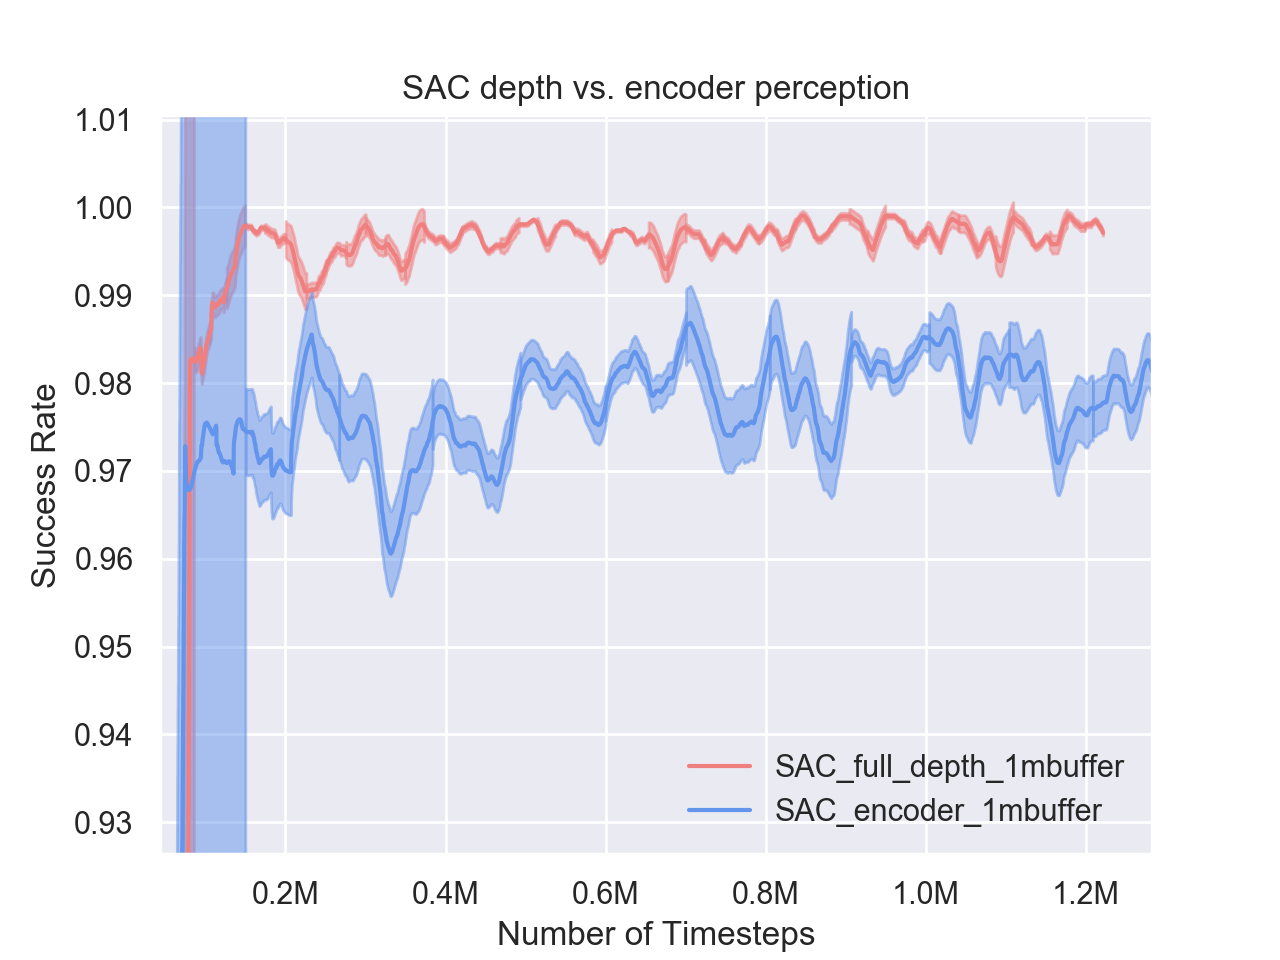
\includegraphics[width=\linewidth]{figures/SACfull/SAC_depth_vs_encoder_perception.png}
        \caption{SAC performance depth versus encoder perception} \label{fig:percep}
    \end{subfigure}%
    \hspace*{\fill}   % maximize separation between the subfigures
    \begin{subfigure}{0.49\textwidth}
        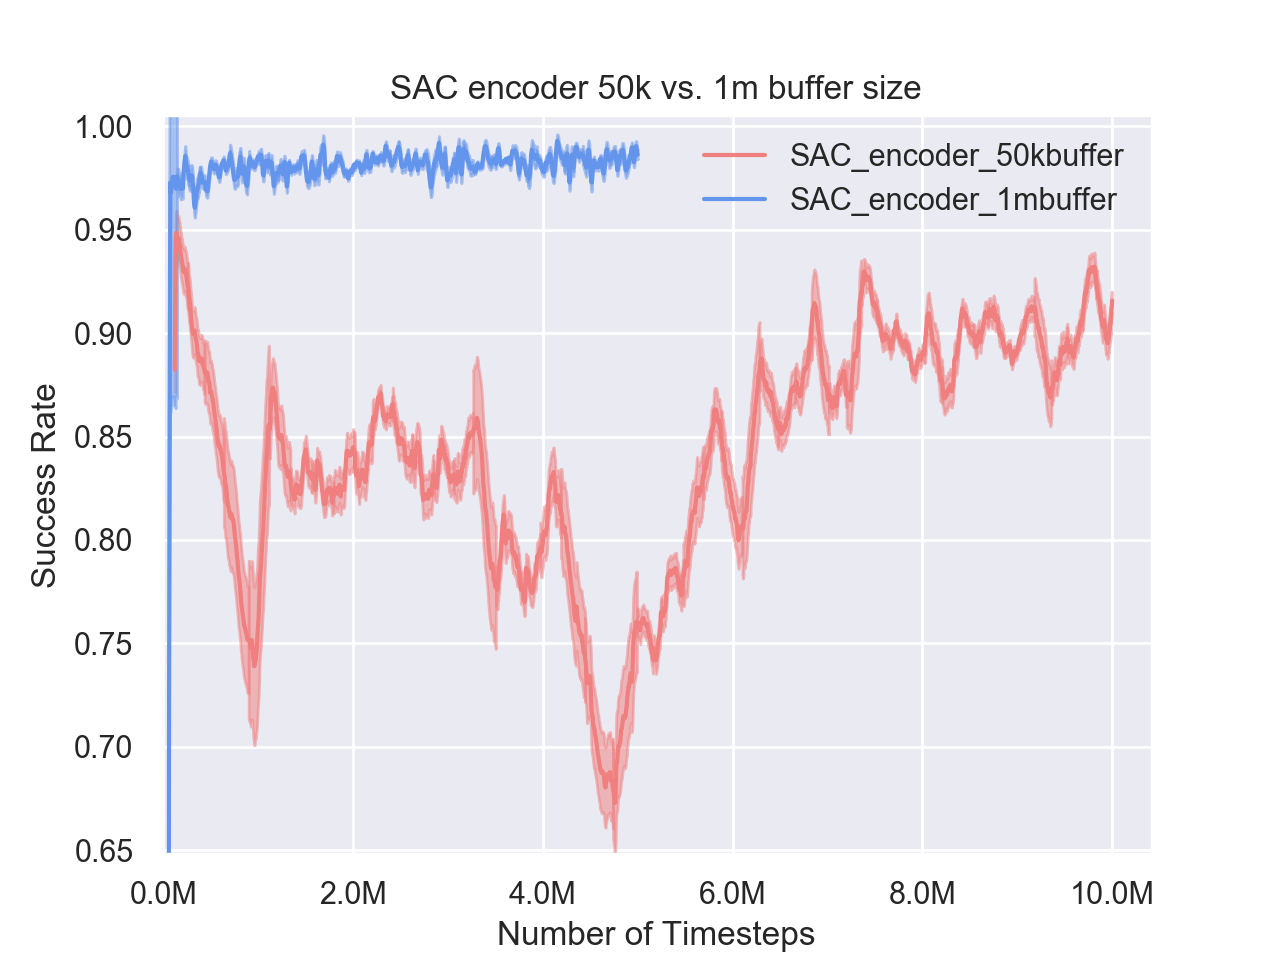
\includegraphics[width=\linewidth]{figures/SACfull/SAC_encoder_50k_vs_1m_buffer_size}
        \caption{SAC performance with encoder perception 50k vs 1m buffer} \label{fig:encbuffer}
    \end{subfigure}%
    \hspace*{\fill}   % maximize separation between the subfigures


\caption{ SAC performance comparison of perception pipelines and buffer size\label{fig:sacperf}}
\end{figure}

\begin{figure}[!htbp]
    \centering
        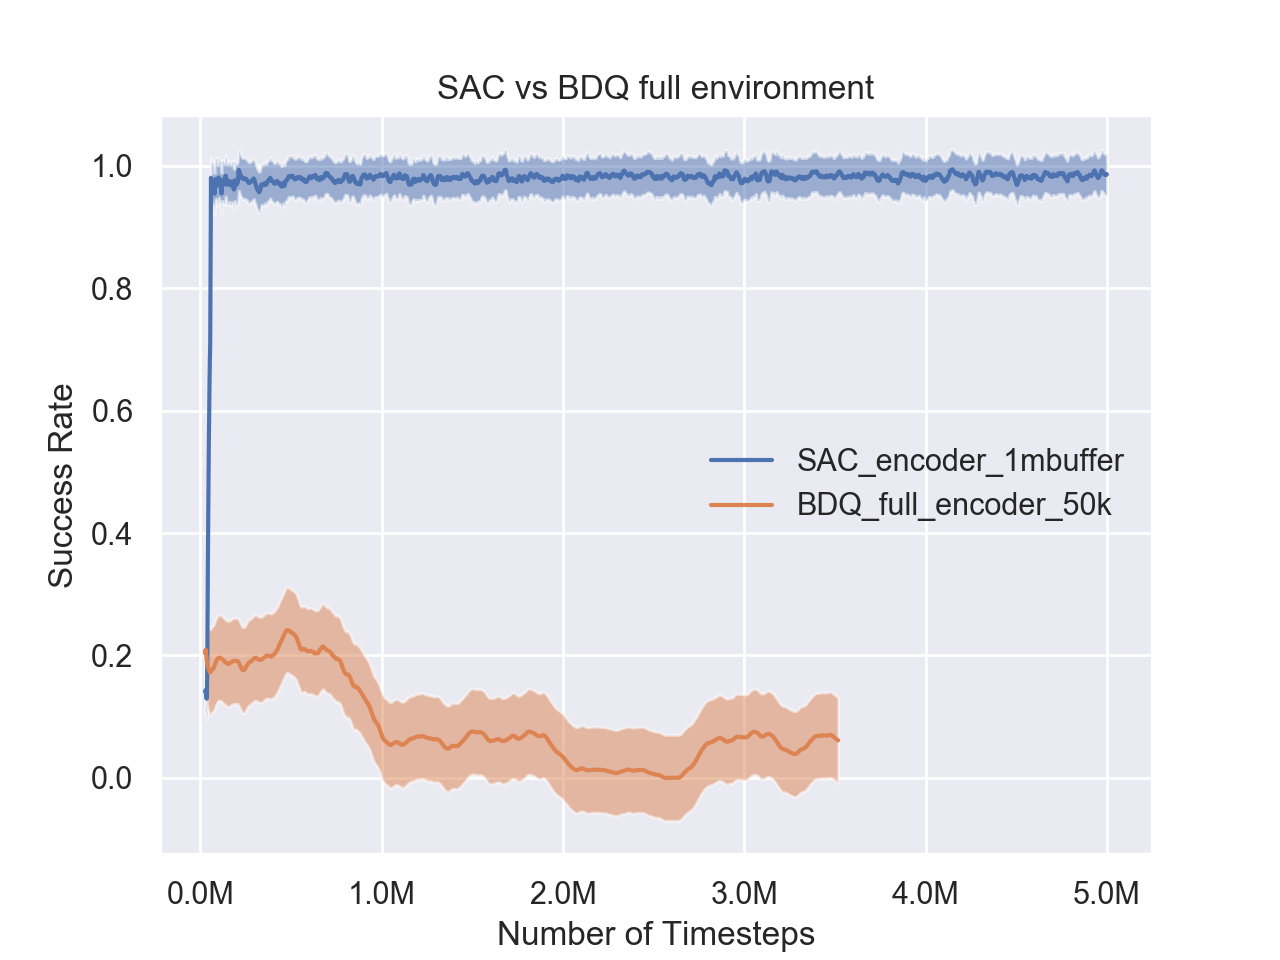
\includegraphics[width=0.7\textwidth]{figures/SACfull/SAC_vs_BDQ_full_environment}
    \caption{SAC compared to BDQ in full environment}
    \label{fig:bdq}
\end{figure}

\begin{figure}[!htbp]
    \centering
        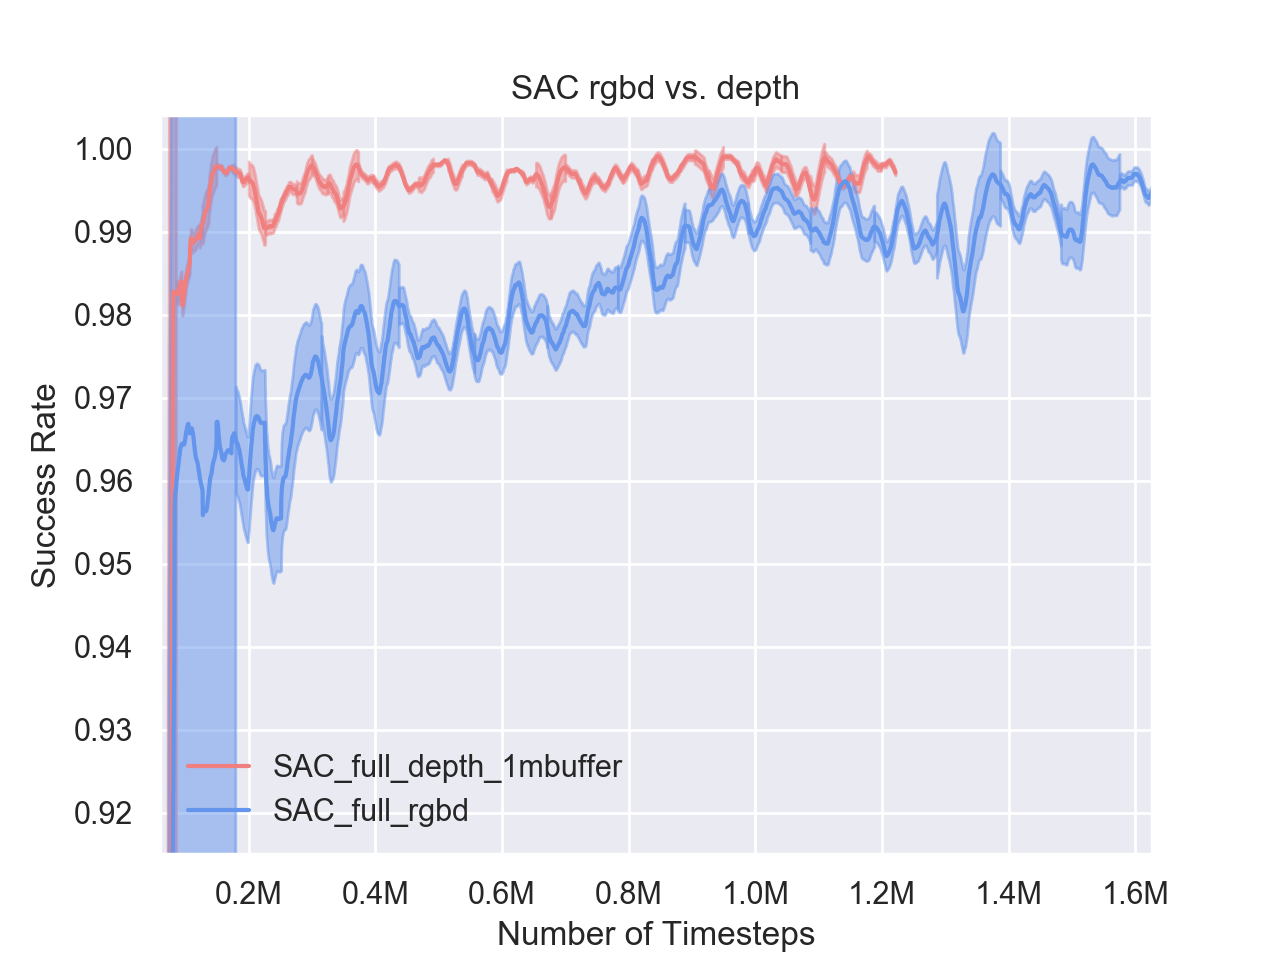
\includegraphics[width=0.7\textwidth]{figures/SACfull/SAC_rgbd_vs_depth}
    \caption{SAC performance RGBD vs. Depth. Shaded region represents the standard deviation.}
    \label{fig:depthvsrgbd}
\end{figure}
